\chapter{Subsistema de control y presentación}\label{chap:control}

\section{Introducción}

El último de los subsistemas que conforma el sistema de medida digital es
el subsistema de control y presentación. Es el subsistema de más alto nivel
de entre los que integran el sistema por interactuar directamente con el
supervisor. El subsistema de control y presentación está constituido por
los bloques de control y presentación propiamente dichos, tal y como
muestra la \cref{fig:subconpre}. Sin embargo, en la práctica estos dos
bloques se mezclan en una misma entidad indivisible, un software que se
ejecuta en el \pc{} anfitrión en el que se encuentra instalada la tarjeta
de adquisición.  Por ser el software que controla el funcionamiento de la
tarjeta \kpci{} pasa a conocerse como \emph{software de control} en este
documento.

\begin{figure}
	\begin{center}
		\includegraphics{gis-pfc-ch3-01.mps}
	\end{center}
	\caption[Subsistema de control y presentación] {Bloques de control
	y presentación dentro del subsistema de control y presentación.}
	\label{fig:subconpre}
\end{figure}

El subsistema de control y presentación constituye la interfaz entre el
supervisor y el sistema de medida, como tal, es una de sus funciones
proporcionar control sobre el sistema al supervisor: ejecutar las órdenes
administradas por el supervisor y gestionar el funcionamiento del resto de
subsistemas. El bloque de control es el encargado de esta actividad y
desempeña las siguientes tareas:

\begin{itemize}
	\item Iniciar y detener la sesión de adquisición.
	\item Interactuar con los drivers de la tarjeta por medio del
		sistema operativo para controlar parámetros de la sesión de
		adquisición como pueden ser, por ejemplo, puertos de
		entrada, modos de adquisición y terminación, o frecuencia
		de muestreo.
	\item Realizar el mantenimiento de los buffers de memoria. Tarea
		que puede dividirse, o consta a su vez, de dos tareas de
		menor complejidad: dar formato a las muestras almacenadas
		en el o los buffers situados en la memoria interna de la
		tarjeta para su comprensión por parte del ordenador
		anfitrión; trasladar las muestras formateadas adecuadamente
		a la memoria del \pc{} para que de ese modo puedan ser
		manipuladas por el usuario administrador.
\end{itemize}

Por su parte, corresponde al bloque de presentación presentar al supervisor
información de utilidad a partir de la señal digital que procede del
subsistema de adquisición. La información debe mostrarse al supervisor para
que pueda interpretarla. En consecuencia, y sometiendo el diseño de la
aplicación de software al criterio del director del PFC, se concluye en
dotar al bloque de presentación con la capacidad de proporcionar la
siguiente información acerca de la señal:

\begin{itemize}
	\item El valor instantáneo cada 250 ms.
	\item El valor medio en el mismo intervalo de tiempo. Este valor
		debe calcularse a partir de las muestras obtenidas en dicho
		periodo a una frecuencia de muestreo que queda a elección
		del supervisor. Debe ser posible seleccionar la frecuencia
		de muestreo desde el propio software de control.
	\item La forma instantánea de la señal, de un fragmento de una
		duración determinada. Debe ser posible también seleccionar
		la duración del fragmento. Simultáneamente debe
		representarse el espectro en frecuencia del fragmento de
		señal que aparece en pantalla.
\end{itemize}

Este capítulo se ha distribuido en dos apartados. En el primero de los
apartados se describe la herramienta empleada en el desarrollo del software
de control. En el segundo se exponen las conclusiones obtenidas al estudiar
el osciloscopio digital como herramienta de referencia en la representación
gráfica de señales. De ese modo se evita explicar el significado del código
correspondiente al software de control línea por línea, puesto que el
lector puede concebir su propia idea del aspecto que adopta el software en
su estadio definitivo de desarrollo. El ejercicio de reflexión pertinente
conduce a una positiva comprensión del proceso que partiendo del diseño
original concluye en el resultado esperado.

% 				( V )
% ______________________________m\"/m______________________________________
%				  '
% El texto comentado aquí abajo debe trasladarse a otra sección del
% capítulo
% _________________________________________________________________________
%
% Se impone una condición de diseño adicional, el software de control debe
% ser poco exigente a fin de que pueda ser ejecutado en un \pc{} que
% disponga de escasos recursos. Para cumplir con dicha condición se propone
% la siguiente solución: limitar la cantidad de datos diferentes
% presentados por pantalla simultáneamente a uno. De ese modo el usuario
% del software debe elegir en cada momento entre el valor instantáneo, el
% valor medio y la forma de la señal y su espectro en frecuencia, y sólo el
% tipo de dato seleccionado se genera reduciendo el coste de procesado.
% Esta solución puede ampliarse incorporando la posibilidad de deshabilitar
% la representación del espectro o de la forma de la señal.
%
% 				 ,._
%				@",_)6
%				 " "

\section{Herramienta de Adquisición de Datos}


\subsection{Introducción}

\psig{matlab} (\emph{MATrix LABoratory}) es la plataforma seleccionada para
el desarrollo del software de control. Es una plataforma de desarrollo bien
conocida en entornos matemáticos y tecnológicos de uso extendido en
universidades y otros centros educativos y de investigación. Encaja en la
descripción de un kit de desarrollo de software (\sig{sdk}) al estar
compuesto por un entorno de desarrollo integrado (\sig{ide}) con editor,
compilador y depurador; y una colección de módulos y extensiones que en
conjunto se comportan como una interfaz de programación de aplicaciones
(\sig{api}).  \matlab{} se caracteriza por emplear un lenguaje propio, el
lenguaje \psig{m}, enfocado a un uso matemático y que se ha diseñado para
simplificar el manejo de datos agrupados en estructuras matemáticas
complejas como son las matrices y los vectores. Los módulos y herramientas
que se incluyen en el \sig{sdk} contribuyen a ampliar su funcionalidad,
convirtiéndolo en un software potente y completo. Estas herramientas
abstraen al desarrollador de implementar por sí mismo en lenguaje \sig{m}
funciones destinadas a realizar operaciones cotidianas como representar
unos datos por pantalla u obtener la \sig{fft} de un vector. Existen
módulos ---o \emph{toolboxes} como se los conoce en inglés--- mantenidos
por la compañía de software, a los que se suman los diseñados por los
propios usuarios, que abundan en la red, disponibles desde la base de datos
dispuesta para ello por la empresa, con lo que las posibilidades son en la
práctica infinitas.  Además \matlab{} cuenta con dos herramientas
fundamentales, muy ligadas al \sig{sdk}, una es \psig{guide}
(\emph{Graphical User Interface Development Environment}), una herramienta
para el desarrollo de interfaces gráficas de usuario (\psig{gui}); y otra
\emph{Simulink}, herramienta que se emplea para realizar todo tipo de
simulaciones.

Las dos razones principales por las que se utiliza \matlab{} son, por un
lado, las facilidades que aporta en la creación de \gui{} y manejo de
señales digitalizadas; y por otro, y aún más importante si cabe, que
incorpora una herramienta denominada \emph{Data Acquisition Toolbox},
nombre que podría traducirse como Herramienta de Adquisición de Datos, en
lo sucesivo \psig{dat}. La \datx{} es una herramienta compuesta por una
biblioteca y un mecanismo para el intercambio de información, que en
conjunto permiten mediante código de alto nivel interactuar directamente
con dispositivos de características similares a las de la tarjeta de
adquisición \kpci{}, y que es convenientemente compatible con ésta tarjeta.
En otras palabras, puede entenderse la \datx{} como una \sig{api} o
interfaz que proporciona al desarrollador las llamadas necesarias para
interactuar directamente con dispositivos de adquisición al tiempo que
abstrae los mecanismos de más bajo nivel que intervienen en el proceso,
descargando al desarrollador de la responsabilidad de implementarlos por él
mismo. Lo que, al fin y al cabo puede resumirse en que en la \datx{} se
implementa el núcleo de lo que se entiende como bloque de control. Al
programarse el software de control empleando los recursos que proporciona
la \datx{}, la herramienta en sí pasa a ser parte fundamental del
subsistema de control y presentación al prestarse como núcleo del bloque de
control. Cobra pues vital importancia en el sistema de medida. En
consecuencia, resulta adecuado un apartado en el que se introduzca la
herramienta al lector. En primer lugar se describen las distintas entidades
que participan en el funcionamiento de la herramienta, justo después se
recoge un subconjunto de las distintas funciones que la \datx{} pone a
disposición del desarrollador ordenadas siguiendo el mismo orden en el que
son requeridas durante la sesión de adquisición de carácter más básico.


\subsection{Componentes de la herramienta}

Los elementos de \matlab{} que juegan un papel suficientemente importante
en el funcionamiento de la \datx{} son los listados en el
\cref{tab:toolcomp}. El diagrama representado en la \vref{fig:toolcomp}
muestra las interdependencias que existen entre los elementos que aparecen
en dicho cuadro.

\begin{table}
	\centering
	\begin{tabulary}{.9\textwidth}{C L}
		\toprule
		Componente & \multicolumn{1}{c}{Propósito} \\
		\midrule
		Ficheros *.m & Se emplean para automatizar la creación de
		objetos dispositivo, adquirir datos, configurar las
		propiedades del dispositivo y la sesión, y evaluar el
		estado de la adquisición y los recursos.\\
		\midrule
		Máquina virtual de adquisición de datos & Almacena objetos
		dispositivo y sus propiedades, controla el almacenamiento
		de los datos adquiridos y controla la sincronización de
		eventos.\\
		\midrule
		Adaptadores & Son la vía de comunicación entre la máquina
		virtual de adquisición de datos y el hardware por la cual
		se transmiten propiedades, datos y eventos.\\
		\bottomrule
	\end{tabulary}
	\caption[Descripción de los componentes de la \datx{}] {Descripción
	de los componentes de la \datx{}.}
	\label{tab:toolcomp}
\end{table}

\begin{figure}
	\begin{center}
		\includegraphics{gis-pfc-ch3-07.mps}
	\end{center}
	\caption[Elementos que intervienen en el funcionamiento de la
	\datx{}]{Elementos que intervienen en el funcionamiento de la
	\datx{}.}
	\label{fig:toolcomp}
\end{figure}

\subsubsection{Objetos dispositivo}

Los objetos dispositivo permiten el acceso a subsistemas específicos del
hardware. Los objetos dispositivo soportados por la \datx{} son los objetos
de entrada analógica o \emph{analog imput objects} (\psig{ai}), los objetos
de salida analógica o \emph{analog output objects} (\psig{ao}) y los
objetos de entrada/salida digital o \emph{digital I/O objects}
(\psig{dio}).

\begin{figure}
	\begin{center}
		\includegraphics{gis-pfc-ch3-08.mps}
	\end{center}
	\caption[Comunicación entre los subsistemas del hardware y los
	objetos dispositivo]{Grafo que representa la comunicación entre los
	subsistemas del hardware y los objetos dispositivo.}
	\label{fig:subsystemsOO}
\end{figure}


\subsection{La sesión de adquisición de datos}

Una sesión completa de adquisición de datos consiste en cinco pasos:

\begin{enumerate}
	\item Crear el objeto dispositivo.
	\item Añadir canales al objeto dispositivo.
	\item Configurar las propiedades del objeto dispositivo y los
		canales añadidos para controlar el comportamiento de la
		aplicación de adquisición de datos.
	\item Adquirir los datos.
	\item Eliminar el objeto dispositivo.
\end{enumerate}

Cada uno de los pasos se detalla en los puntos subsiguientes.


\subsubsection{Crear el objeto dispositivo}

Para crear un objeto dispositivo, se debe llamar a la función de creación
apropiada o constructor. Como se muestra en el \cref{tab:constructors}, los
constructores reciben un nombre particular en función del tipo de objetos
dispositivo que crean. Para iniciar una sesión de adquisición de datos
analógicos es necesario un comando como el siguiente, \func{analoginput}
\func{(`adaptador', ID)}. Un ejemplo extraído del código fuente de la
aplicación de control muestra cómo hacerlo en el \cref{cod:constructor}.

\begin{table}
	\centering
	\begin{tabular}{l >{\tt}l}
		\toprule
		\multicolumn{1}{c}{Tipo de subsistema} %
		& \multicolumn{1}{c}{\rm Constructor} \\
		\midrule
		Entrada analógica & analoginput(`adaptador', ID); \\
		\midrule
		Salida analógica & analogoutput(`adaptador', ID); \\
		\midrule
		Entrada / Salida digital & digitalio(`adaptador', ID); \\
		\bottomrule
	\end{tabular}
	\caption[Tipos de constructor en función del objeto dispositivo
	creado]{Tipos de función de creación de acuerdo con el tipo
	subsistema al que se orienta el objeto dispositivo creado.}
	\label{tab:constructors}
\end{table}

\begin{lstlisting}[style=displayed, caption={[Método a seguir para crear un
	objeto dispositivo] {Método que evalúa la existencia de un objeto
	dispositivo previo a la llamada de la aplicación, en caso positivo
	lo hereda para su uso posterior, de lo contrario crea uno
	nuevo.}}, label={cod:constructor}]
	set(handles.ai, 'TriggerType', 'Immediate', 'TimerFcn', '', ...
	handles.ai = [];

	if ~isempty(daqfind)
		oldObj = daqfind;

		for i = 1:length(oldObj);
			auxStr = daqhwinfo(oldObj(i));
			auxNum = findstr(' ', auxStr.DeviceName) - 1;
			if strcmp('KPCI-3108', ...
				auxStr.DeviceName(1:auxNum)) && ...
				strcmpi('analoginput', auxStr.SubsystemType);
				handles.ai = oldObj(i);
				warning('El dispositivo esta en uso.');
				break
			end
		end

	end

	if isempty(handles.ai)
		try
			handles.ai = analoginput('keithley');
		catch
			errordlg('No pudo crearse el manejador de dispositivo.');
		end
	end
\end{lstlisting}

El argumento \func{id} es un indicador de dispositivo hardware. Se trata de
un argumento opcional para tarjetas de sonido con \func{id} 0. El argumento
\func{adaptador} requiere el nombre del adaptador de dispositivo hardware.
A continuación, en el \cref{tab:adaptors} se muestra una relación con los
adaptadores de dispositivo cuyo uso es más frecuente y el nombre de
adaptador que debe introducirse como argumento de la llamada a
\func{analoginput}. Por conveniencia se ha añadido Keithley a esta lista.

\begin{table}
	\centering
	\begin{tabular}{l >{\tt\qquad}l}
		\toprule
		\multicolumn{1}{c}{Fabricante de Hardware} %
		& \multicolumn{1}{c}{\rm Nombre de adaptador} \\
		\midrule
		Advantech & advantech \\
		\midrule
		Measurement Computing & mcc \\
		\midrule
		National Instruments & nidaq \\
		\midrule
		Parallel port & parallel \\
		\midrule
		Microsoft Windows & winsound \\
		\midrule
		Keithley Instruments, Inc. & keithley \\
		\bottomrule
	\end{tabular}
	\caption[Valores que puede adoptar el argumento
	\func{adaptador}.]{Valores que puede adoptar el argumento
	\func{adaptador} necesario en la llamada a \func{analoginput}.}
	\label{tab:adaptors}
\end{table}


\subsubsection{Añadiendo canales}

Antes de poder utilizarse, deben añadirse canales al objeto dispositivo.
Para ello, debe emplearse la función \func{addchannel}. Puede pensarse en
un objeto dispositivo como un contenedor de grupos de canales y en los
canales añadidos a un objeto dispositivo como un grupo de canales. Si se
desean añadir dos canales al objeto dispositivo \func{objeto} puede
utilizarse la siguiente llamada \func{cans = addchannel(objeto, 1:2);}.


\subsubsection{Configurando propiedades}

Puede controlarse el comportamiento de una sesión de adquisición de datos o
de una aplicación creada con tal propósito configurando las propiedades de
los objetos dispositivo que intervienen en el proceso de adquisición y de
los canales que dicho objeto contiene. Estas son las reglas principales en
la configuración de propiedades desde la \datx{}.

\begin{itemize}
	\item Los nombres de las propiedades pueden escribirse en
		mayúsculas, minúsculas o combinación de ambas.
	\item Los nombres de las propiedades pueden abreviarse como se
		mostrará a continuación. % Hay que confirmar que se
		% explican las reglas de abreviatura
	\item La función \func{set} aplicada a un objeto dispositivo
		---\func{set(objeto)}--- devuelve todas las propiedades
		configurables de ese objeto. Si se llama a \func{set}
		utilizando como argumento un canal ---\func{set(objeto.}
		\func{.Channel(índice)}---, la función devolverá todas las
		propiedades configurables de dicho canal.
	\item La función \func{get} devuelve todas las propiedades de un
		canal u objeto y el valor que toman en el momento en el que
		se llama a la función si se emplea como único argumento
		dicho canal u objeto ---\func{get(objeto)},
		\func{get(objeto.Channel(índice)}---.  \end{itemize}

Se distinguen dos tipos de propiedades distintas asociadas a los canales
contenidos en un objeto dispositivo.

\begin{description}
	\item[Propiedades comunes] Son aquellas propiedades que se aplican
		todos los canales pertenecientes a un mismo objeto
		dispositivo.
	\item[Propiedades de canal] A diferencia de las propiedades
		comunes, las propiedades de canal pueden configurarse
		individualmente por canal.
\end{description}

Dentro de las propiedades comunes de los canales existen las
\emph{propiedades básicas}, que se aplican a todos los subsistemas de un
determinado tipo (\textsc{ai, ao, dio}); y \emph{propiedades específicas de
dispositivo} aplicables únicamente al hardware específico que se está
empleando.

Existen tres formas de configurar u obtener el valor de una propiedad:
utilizando las funciones \func{set} y \func{get}; empleando la notación de
punto; o recurriendo a los nombres indexados.

\begin{itemize}
	\item La sintaxis de las funciones \func{get} y \func{set} es
		similar a la empleada en la herramienta de \matlab{}
		\emph{Handle Graphics}.

		\begin{lstlisting}[gobble=16]
			out = get(objeto, `SampleRate');
			set(objeto, `SampleRate', 11025)
		\end{lstlisting}

	\item La notación de punto se emplea del siguiente modo:

		\begin{lstlisting}[gobble=16]
			out = objeto.SampleRate;
% 			objeto.SampleRate = 11025;
		\end{lstlisting}

	\item Por último, los nombres indexados permiten asociar un nombre
		descriptivo a cada canal. Por ejemplo para asociar el
		nombre \func{Can1} con el primer canal contenido en
		\func{objeto} debe procederse como se enuncia a
		continuación.

		\begin{lstlisting}[gobble=16]
			set(objeto.Channel(1), `ChannelName', `Can1');
			out = objeto.Can1.UnitsRange;
			objeto.Can1.UnitsRange = [0, 10];
		\end{lstlisting}

\end{itemize}


\subsubsection{Adquisición de datos}

La adquisición de datos puede dividirse en tres tareas básicas: iniciar el
objeto dispositivo; registrar datos y detener el objeto dispositivo.

La función que se utiliza para iniciar un objeto dispositivo es la función
\func{start}, p.e. para iniciar el objeto dispositivo \func{objeto} habría
que llamar a la función de esta forma \func{start(objeto)}. Tras iniciar un
objeto su propiedad \textsf{Running} pasa de manera automática al valor
\textsf{On}.

No obstante haber iniciado el dispositivo, este no empieza a registrar
datos hasta que no ocurre un trigger o disparo. Hay diversos tipos de
trigger, en el \vref{tab:triggers} se muestran aquellos soportados por
todos los dispositivos. Tras un trigger el dispositivo hardware inicia la
adquisición de datos y la propiedad \textsf{Logging} del objeto dispositivo
asociado conmuta al estado \textsf{On}.

\begin{table}
	\centering
	\begin{tabulary}{.9\linewidth}{>{\sf}c L}
		\toprule
		{\rm Tipo de disparo} & \multicolumn{1}{c}{Descripción} \\
		\midrule
		Inmediato & El disparo ocurre justo después de la llamada a
		\func{start}. Este es el tipo de trigger predeterminado. \\
		\midrule
		Manual & El disparo ocurre después de llamar manualmente a
		la función \func{trigger}. \\
		\midrule
		Software & El disparo sucede cuando se detecta una señal
		que satisface una determinada condición especificada de
		antemano. El objeto dispositivo debe disponer de más de un
		canal que hará las veces de la señal de disparo. Debe
		especificarse, como es obvio, que canal actúa como fuente
		del disparo. \\
		\midrule
		Reloj interno & Por añadidura, la \kpci{} cuenta con la
		posibilidad de recibir el disparo de la fuente de reloj
		interna. \\
		\bottomrule
	\end{tabulary}
	\caption[Tipos de disparo soportados por el hardware compatible con
	\matlab{}]{Tipos de disparo soportados por el hardware compatible
	con \matlab{} y una breve descripción de los mismos.}
	\label{tab:triggers}
\end{table}

Por último, existen tres causas por las que un objeto dispositivo puede
detenerse: \matlab{} detiene un objeto dispositivo iniciado una vez
obtenidos los datos precisados por el usuario; al ocurrir un error de
tiempo de ejecución en relación con la actividad de un objeto dispositivo
éste es detenido también; y tan sólo resta el método manual, que consiste
en llamar a la función \func{stop}, por ejemplo \func{stop(objeto)}.

Como se ha mencionado la máquina virtual de adquisición de datos registra y
controla los datos que extrae de un objeto dispositivo. Un usuario puede
acceder a esos datos de dos formas diferentes:

\begin{itemize}
	\item La primera de ellas se conoce como previsualizar los datos.
		Se emplea con ese propósito la función \func{peekdata}. Si,
		por ejemplo, se quisiese previsualizar 1000 muestras
		obtenidas con el objeto dispositivo \func{objeto}, la
		llamada a \func{peekdata} sería la siguiente: \func{out =
		peekdata(objeto, 1000);}. La función \func{peekdata}
		devuelve el control a \matlab{} de inmediato y no elimina
		los datos previsualizados de la máquina virtual de
		adquisición.
	\item En cualquier momento tras adquirir datos mediante un objeto
		dispositivo estos pueden extraerse de la máquina virtual de
		adquisición mediante la función \func{getdata}. Partiendo
		del ejemplo anterior, si se desea extraer 1000 muestras
		procedentes del objeto dispositivo \func{objeto}, esta es
		la llamada adecuada \func{out = getdata(objeto, 1000);}. Al
		contrario que la función \func{peekdata}, \func{getdata} no
		devuelve el control a \matlab{} hasta haber extraído todas
		las muestras solicitadas. Es evidente que las muestras
		extraídas dejarán de estar disponibles en la máquina
		virtual de adquisición.
\end{itemize}

Es importante señalar que en cualquiera de los procedimientos descritos
intentar acceder a más datos de los obtenidos en un determinado momento
causará un error que detendrá el funcionamiento del objeto dispositivo.


\subsubsection{Eventos y Callbacks}

Puede decirse que un evento sucede en un determinado instante después de
que una cierta condición se cumple. A menos que ocurra un error, en todas
las sesiones de adquisición de datos debe producirse un evento de inicio,
uno de disparo y uno de parada. Puede accederse a la información que
transporta un evento mediante la propiedad \textsf{EventLog}:

\begin{lstlisting}
	Events = ai.EventLog;
	EventTypes = {Events.Types}
	EventTypes =
		`Start'    `Trigger'	`Stop'
\end{lstlisting}

Cuando se produce un evento, puede ejecutarse una función de
\emph{callback}. Es posible seleccionar una función para un callback
especificando como valor de la propiedad asociada a dicho callback el
nombre de la función (si ésta se encuentra en el mismo fichero *.m que
contiene el código que ejecuta la aplicación que realiza la adquisición de
datos), o el nombre del fichero *.m con el código de la función. Así mismo,
pueden pasarse argumentos de entrada a la función de callback asignándolos
a la mencionada propiedad.

Por ejemplo, los siguientes comandos configuran \func{objeto} de forma que
la función \func{datadqcallback} se ejecute desde el fichero cuyo nombre
está compuesto por una raíz idéntica al nombre de la función y con
extensión *.m, cuando se produzca un evento de trigger o de parada durante
la actividad del objeto dispositivo. Además se pasa como argumento de la
función el valor de la propiedad \textsf{Running} de \func{objeto} en el
momento del callback.

\begin{lstlisting}
	set(objeto, `TriggerFcn', @datadqcallback, objeto.Running)
	set(objeto, `StopFcn', @datadqcallback, objeto.Running)
\end{lstlisting}

Un segundo ejemplo, este extraído del código fuente de la aplicación de
control muestra como pasar argumentos a la función de callback y cuál es la
sintaxis de la definición de la misma en el \cref{cod:callback}.

\begin{lstlisting}[style=displayed, caption={[Configuración de
	\emph{callback}]{Configuración de \emph{callback} para responder a
	eventos en la sesión de muestreo, la función de \emph{callback}
	recibe un argumento.}}, label={cod:callback}]
	set(handles.ai, 'TriggerType', 'Immediate', 'TimerFcn', '', ...
		'SamplesAcquiredFcn', {@localDaqCallback, gcbo});

				[...]

	function localDaqCallback(obj, event, hObject)
		handles = guidata(hObject);
		EventType = event.Type;

		switch lower(EventType)
			case 'samplesacquired'

				[...]

			case 'timer'

				[...]

		end
\end{lstlisting}

\subsubsection{Suprimiendo y borrando las trazas de los objetos dispositivo}

La función \func{delete} elimina el objeto dispositivo especificado de la
máquina virtual de adquisición, pero no del espacio de trabajo (espacio
reservado a las variables de trabajo) de \matlab{},
---\func{delete(objeto)}---. Tras una llamada semejante \func{objeto} sigue
apareciendo en el espacio de trabajo de \matlab{}, pero se trata de un
objeto inválido desde el momento en el que deja de encontrarse ligado al
hardware. Deben suprimirse los objetos dispositivo faltos de validez con el
comando \func{clear}, p.e., \func{clear objeto}.

Si se suprime un objeto dispositivo del espacio de trabajo de \matlab{} no
deja de existir en la máquina virtual. Para poder recuperar objetos
borrados accidentalmente puede utilizarse la función \func{daqfind}.

\begin{lstlisting}
	out = daqfind;	ai = out(1);
\end{lstlisting}


\section{Diseño conceptual del software}\label{sec:softdesign}

\textsc{Matlab} y la \datx{} simplifican en gran medida la tarea de
implementar el bloque de control y la interfaz gráfica de usuario, por
tanto, el último reto importante que debe afrontarse en el desarrollo del
software de control es programar el mecanismo mediante el cual ha de
representarse la señal en pantalla. Es sencillo mostrar por pantalla datos
numéricos o representar la \sig{fft} de una señal gracias a las utilidades
de que dispone \matlab{}, representar una señal en <<tiempo real>> es algo
más complejo. Al fijar los objetivos del \sig{pfc} se especifica que debe
poder utilizarse el sistema de medida para visualizar señales como si se
tratase de un osciloscopio digital. La principal complicación que existe al
programar un osciloscopio digital en software radica en definir las metas
de programación y no en escribir el código. Esto sólo puede lograrse tras
estudiar en profundidad el modelo, después de comprender perfectamente su
comportamiento y de ese modo poder traducir sus principales rasgos de
conducta en metas sencillas. En este apartado se exponen brevemente las
conclusiones extraídas tras estudiar el osciloscopio digital como modelo
para el software de control.


\subsection{El osciloscopio digital}\label{subsec:digosc}

El osciloscopio digital es un dispositivo que se emplea para visualizar
señales, es el sucesor de otros instrumentos como el oscilógrafo y el
osciloscopio analógico. Algo importante a tener en cuenta cuando se estudia
el osciloscopio digital es que se ha diseñado para conseguir un resultado
similar al que se espera de un osciloscopio analógico. La diferencia entre
uno y otro reside en la forma en la que se genera un barrido, el
osciloscopio analógico dibuja la señal sobre la marcha mientras que el
osciloscopio digital digitaliza y almacena la señal digital en memoria
antes de representar. Un barrido es básicamente una imagen de la señal que
abarca toda la pantalla del osciloscopio, se llama así porque el haz de
electrones que emite el tubo de rayos catódicos de un osciloscopio
analógico barre literalmente el monitor para formar la imagen (que no es
más que la imprenta dejada en el monitor por la acción del fósforo). Pero
en los osciloscopios digitales no hay barridos como tal, en realidad los
osciloscopios digitales utilizan monitores \sig{led} en los que los
distintos puntos de luz se apagan, o se encienden, o cambian de color,
accionados por una señal de control. Cuando muchos barridos se suceden
rápidamente se crea la sensación de que la representación de la señal se
mueve, aunque no es así, y en los osciloscopios digitales la representación
es estrictamente estática. Pero el resultado final es muy similar, a
efectos prácticos es el mismo, pues el ojo humano no es capaz de percibir
la diferencia y eso en la práctica significa que esa diferencia no existe.
Pero si existe diferencia, y esa diferencia se nota en algunos aspectos
relacionados con el funcionamiento del osciloscopio digital. Usualmente
tanto los osciloscopios digitales como los analógicos hacen barridos
disparados de la señal, esto es, empiezan a representar la señal al
detectar un evento ---un flanco de subida o de bajada o similar--- en una
señal de referencia que puede y acostumbra a ser la propia señal con la que
se trabaja. De esa forma se consigue alinear todas las capturas o ciclos de
la señal en fase unos con otros y con la señal. Si no se dispara resulta
muy difícil observar la señal con el osciloscopio, especialmente si se
trata de una señal aperiódica, porque los distintos ciclos representados se
superponen y es difícil distinguir la señal correctamente. La diferencia
entre los osciloscopios analógicos y digitales se manifiesta especialmente
en que el osciloscopio analógico empieza a representar la señal cuando
detecta el evento y el usuario puede ver como evoluciona, sin embargo, el
osciloscopio digital empieza a \emph{muestrear} cuando observa el evento y
no representa hasta que tiene muestras suficientes como para abarcar toda
la dimensión temporal representada en el monitor, es ahí donde se hace
evidente un retardo. Imagínese la siguiente situación por ejemplo: se
trabaja con una señal que oscila lentamente y se configura la escala
temporal del osciloscopio para poder observar un periodo completo de la
señal en pantalla, como la señal es lenta su periodo es largo, entonces
llega el evento y en el osciloscopio analógico empieza a verse la señal
apareciendo lentamente desde el margen izquierdo de la pantalla, sin
embargo, en el osciloscopio digital no se ve nada y el retardo se hace
visible y molesto. El retardo que se produce en situaciones como la
expuesta, en las que trata de observarse evoluciones lentas de una señal,
dificulta el uso de los osciloscopios, pero especialmente el uso de los
osciloscopios digitales. Para paliar los efectos del retardo, el
osciloscopio digital aprovecha que puede representar los datos que tiene en
memoria de otras formas diferentes y, cuando la escala temporal de la
representación se configura por encima de un nivel de umbral, simula el
comportamiento de los osciloscopios analógicos. En lugar de hacer barridos
de la señal, actualiza la pantalla en ciclos cortos añadiendo a la
representación fragmentos muy pequeños de señal, cortos en comparación con
la dimensión temporal representada en el eje de abscisas. Los fragmentos
tienen una duración igual al periodo con el que se refresca el monitor, que
es un periodo de refresco fácilmente asumible por el osciloscopio dada la
configuración de la escala temporal, pero que es muy difícil de seguir por
parte del ojo humano. Cuando opera de este modo, el osciloscopio digital
simula que la señal va desplazándose de derecha a izquierda, y el resultado
es idéntico al que muestran los osciloscopios digitales. Las
\vref{fig:sigmodcont,fig:firmodcont,fig:desmodcont} ilustran este
comportamiento.

\begin{figure}
	\begin{center}
		\includegraphics{gis-pfc-ch3-04.mps}
	\end{center}
	\caption[Señal analógica, representación continua]{Señal analógica
	vista desde la sonda del osciloscopio, se han marcado los instantes
	en los que se refresca el monitor del osciloscopio.}
	\label{fig:sigmodcont}
\end{figure}

\begin{figure}
	\begin{center}
		\includegraphics{gis-pfc-ch3-05.mps}
	\end{center}
	\caption[Evolución que sufre la representación]{Evolución de la
	representación cuando aún no abarca la dimensión horizontal del
	monitor.}
	\label{fig:firmodcont}
\end{figure}

\begin{figure}
	\begin{center}
		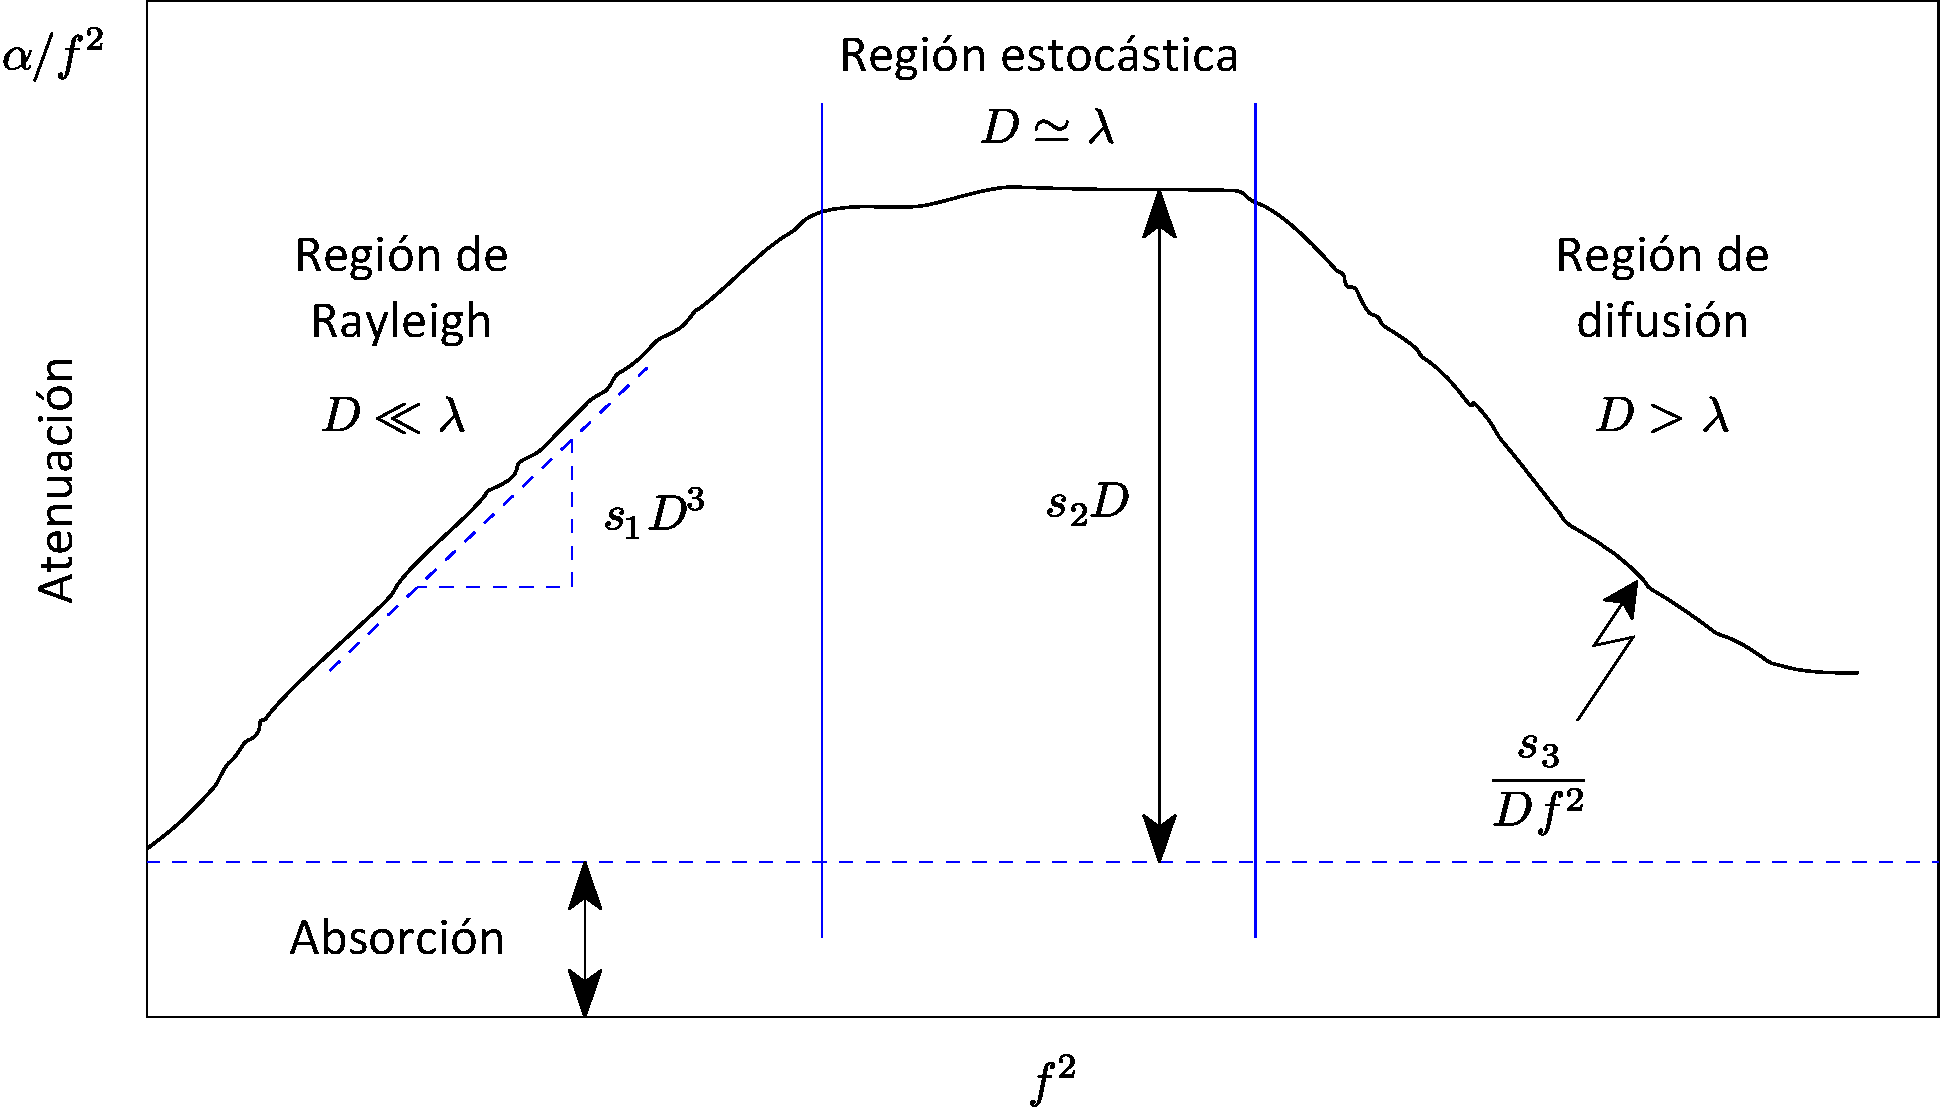
\includegraphics{gis-pfc-ch3-06.mps}
	\end{center}
	\caption[Desplazamiento que experimenta la
	representación]{Desplazamiento que experimenta la representación
	una vez ocupa toda la pantalla del osciloscopio.}
	\label{fig:desmodcont}
\end{figure}

\subsubsection{Barrido disparado}

Implementar un barrido disparado mediante software directamente en la
aplicación de control es complicado teniendo en cuenta la configuración del
sistema de medida. Podría hacerse por hardware, sería necesario generar una
señal de reloj mediante un circuito externo. El circuito requiere de tres
componentes, uno que genera un tren de pulsos rectangulares de frecuencia
100 kHz que se activa y se detiene por flanco de bajada o subida y que
marca el muestreo, otro que genera el flanco que activa el tren de pulsos
cuando la señal de trabajo efectúa una transición de tensión negativa a
tensión positiva y, por último, otro que genera el flanco que detiene el
tren de pulsos. Como señal que detiene el tren de pulsos es necesario un
tren de flancos, pulsos estrechos, cuyo periodo depende de la escala
temporal de la ventana donde se representa la señal. Dependiendo de la
configuración de este parámetro puede cambiarse el valor de tensión que
sale por uno de los puertos de salida analógica de la \kpci{}, y en función
de esta tensión generar una señal en la que el \emph{duty cycle} varía y la
duración del estado alto se mantiene. El flanco que detiene el muestreo
puede monitorizarse para averiguar cuando debe la aplicación extraer las
muestras del buffer de memoria asociado a la tarjeta y debe empezar a
procesarlas. La señal de reloj debe pasarse a la tarjeta por el puerto
\textsc{j1}, puerto que puede utilizarse como fuente de reloj hardware
externo, y debe configurarse la tarjeta apropiadamente mediante las
propiedades del objeto dispositivo correspondiente en \matlab{}.

Diseñar el circuito y realizar la configuración correspondiente requiere de
un gran esfuerzo por lo que el problema de implementar barridos por disparo
en el software de control se ha atajado empleando una solución aproximada.
En lugar de empezar a muestrear a partir de un evento, de un pulso o de un
flanco en una señal auxiliar o en la propia señal, se muestrea la señal, y
cuando ha transcurrido el suficiente tiempo como para disponer de bastantes
muestras como para cubrir dos ventanas temporales (en este documento se
llama ventana temporal al tiempo que representa el eje de tiempos en cada
momento), entonces se procesan las muestras y además de eliminar la
componente en continua se detectan los nulos de la señal. Después se alinea
el más próximo de los nulos a la muestra central del intervalo con el cero
del plano cartesiano. De esa forma todas las capturas de la señal aparecen
alineadas. Las \cref{fig:sigmodtri,fig:repmodtri} muestran cual es el
resultado de utilizar este algoritmo.

\begin{figure}
	\begin{center}
		\includegraphics{gis-pfc-ch3-02.mps}
	\end{center}
	\caption[Representación de barridos por disparo]{En esta figura se
	muestran las distintas ventanas que intervienen en la solución
	aproximada utilizada para implementar la representación de barridos
	activados por disparo en el software de control. Puede apreciarse
	la información que se descarta en cada ciclo.}
	\label{fig:sigmodtri}
\end{figure}

\begin{figure}
	\begin{center}
		\includegraphics{gis-pfc-ch3-03.mps}
	\end{center}
	\caption[Representación del fragmento de señal]{Fragmento de señal
	representado centrado en el cero del plano cartesiano.}
	\label{fig:repmodtri}
\end{figure}

El coste que se deriva de utilizar un algoritmo como este para obtener
barridos disparados de la señal es la información que se descarta en cada
ciclo, al desplazar la señal todo lo que queda fuera de la ventana no se
representa, con lo que parte de la información capturada es descartada. En
la \cref{fig:sigmodtri} puede observarse el instante $t_0$, instante en el
que empieza el proceso de adquisición, el instante $t_0 + T$ que representa
el momento en el que este proceso termina. Por tanto, el fragmento de señal
contenido entre estos dos instantes se encuentra digitalizado y almacenado
en memoria en el momento en que empiezan a procesarse las muestras,
inmediatamente después de $t_0 + T$. Sin embargo, después de desplazar la
señal todo aquello que queda fuera de la ventana temporal se descarta y
nunca llega a representarse. Además durante el tiempo en el que el software
procesa y representa la señal digital, desde $t_0 + T$ hasta $t_1$, no se
muestrea, por lo que el fragmento de señal que transcurre en esos instantes
también pasa inadvertido al usuario. Todo ello puede contribuir a que
ciertos eventos ocurridos en la señal se pierdan ocasionalmente, sin
embargo, esta solución ha dado hasta el momento muy buenos resultados, tal
y como se demuestra en el \cref{chap:part1conclusions}.
